%%%%%%%%%%%%%%%%%%%%%%%%%%%%%%%%%%%%%%%%%
% Journal Article
% LaTeX Template
% Version 1.3 (9/9/13)
%
% This template has been downloaded from:
% http://www.LaTeXTemplates.com
%
% Original author:
% Frits Wenneker (http://www.howtotex.com)
%
% License:
% CC BY-NC-SA 3.0 (http://creativecommons.org/licenses/by-nc-sa/3.0/)
%
%%%%%%%%%%%%%%%%%%%%%%%%%%%%%%%%%%%%%%%%%

%----------------------------------------------------------------------------------------
%	PACKAGES AND OTHER DOCUMENT CONFIGURATIONS
%----------------------------------------------------------------------------------------

\documentclass[twoside]{article}

% IEEE conference procedings template
%\documentclass[conference]{IEEEtran}
%\hyphenation{op-tical net-works semi-conduc-tor}

\usepackage{lipsum} % Package to generate dummy text throughout this template

\usepackage[sc]{mathpazo} % Use the Palatino font
\usepackage[T1]{fontenc} % Use 8-bit encoding that has 256 glyphs
%\linespread{1.05} % Line spacing - Palatino needs more space between lines
\usepackage{microtype} % Slightly tweak font spacing for aesthetics

\usepackage[hmarginratio=1:1,top=32mm,columnsep=20pt]{geometry} % Document margins
\usepackage{multicol} % Used for the two-column layout of the document
\usepackage[hang, small,labelfont=bf,up,textfont=it,up]{caption} % Custom captions under/above floats in tables or figures
\usepackage{booktabs} % Horizontal rules in tables
\usepackage{float} % Required for tables and figures in the multi-column environment - they need to be placed in specific locations with the [H] (e.g. \begin{table}[H])
\usepackage{hyperref} % For hyperlinks in the PDF

\usepackage{lettrine} % The lettrine is the first enlarged letter at the beginning of the text
\usepackage{paralist} % Used for the compactitem environment which makes bullet points with less space between them

\usepackage{abstract} % Allows abstract customization
\renewcommand{\abstractnamefont}{\normalfont\bfseries} % Set the "Abstract" text to bold
\renewcommand{\abstracttextfont}{\normalfont\small\itshape} % Set the abstract itself to small italic text

\usepackage{titlesec} % Allows customization of titles
\renewcommand\thesection{\Roman{section}} % Roman numerals for the sections
\renewcommand\thesubsection{\Roman{subsection}} % Roman numerals for subsections
\titleformat{\section}[block]{\large\scshape\centering}{\thesection.}{1em}{} % Change the look of the section titles
\titleformat{\subsection}[block]{\large}{\thesubsection.}{1em}{} % Change the look of the section titles

\usepackage{fancyhdr} % Headers and footers
%\pagestyle{fancy} % All pages have headers and footers
%\fancyhead{} % Blank out the default header
%\fancyfoot{} % Blank out the default footer
%\fancyfoot[RO,LE]{\thepage} % Custom footer text

\usepackage{amsmath,amssymb}
\usepackage{graphicx}

\newtheorem{theorem}{Theorem}
\newtheorem{corollary}{Corollary}[theorem]
\newtheorem{lemma}{Lemma}
\newenvironment{proof}[1][Proof]{\begin{trivlist}
		\item[\hskip \labelsep {\bfseries #1}]}{\end{trivlist}}
\newtheorem{case}{Case}

\usepackage[colorinlistoftodos]{todonotes}
%----------------------------------------------------------------------------------------
%	TITLE SECTION
%----------------------------------------------------------------------------------------

\title{\vspace{-15mm}\fontsize{24pt}{10pt}\selectfont\textbf{Data Freshness Over-Engineering: Formulation and Basic Results}} % Article title

\author{
\large
\textsc{Dagaen Golomb}\\[2mm] % Your name
\normalsize University of Pennsylvania \\ % Your institution
\vspace{-5mm}
}
\date{}

%----------------------------------------------------------------------------------------

\begin{document}

\maketitle % Insert title

\thispagestyle{fancy} % All pages have headers and footers

%----------------------------------------------------------------------------------------
%	ARTICLE CONTENTS
%----------------------------------------------------------------------------------------

%\begin{multicols}{2} % Two-column layout throughout the main article text

\section{Introduction}

There are many applications where a task needs to consume data in order to perform its duties. In real-time systems, this input is often sensor data that is crucial for determining the behavior of the system. Input may also be from the output of other tasks. In these types of systems, there is usually an explicit or implicit timeliness requested for this data. The relevance of a computation can be intuitively evaluated by the age, or "freshness," of the data that was used during the computation.

Traditionally, tasks have been over-engineered to provide fresh data. Imagine a task that must perform some computation on data, produced by another task, every one second. Should the task producing the required data run every second? 500 milliseconds? 100 milliseconds? How is the designer to decide? In these situations, engineers may err on the side of caution and choose to produce the input data faster than necessary, which they then need to test in order to evaluate safety. For example, A task that reads a sensor value and forwards it to another task may be dispatched fifty times a second even though the consuming task only needs data younger than one tenth of a second for safety. While this is presumably safe, it reduces the efficiency (and possibly schedulability) of the system, and there is no formal method for us to decide if this value is safe regardless. This leads to more dependence on testing. As Microsoft acknowledges, overenginnering alway leads to wasted effort \cite{CODEMINE}. This often leads to several cycles of parameter tuning in order to ensure the safety and efficiency of the system without ultimately guaranteeing optimal efficiency, as noted by several others in the field \cite{BiniNatale,SetoLehoczkySha,ChantemWangLemmonHu,BelwalCheng}. This paper outlines a formalization of this over-engineering strategy and presents results for choosing the period of input tasks given little information about the underlying system.
\section{Motivation}

Something goes here.
\section{Goal}

In broad terms, the goal we wish to achieve is for the input of a given task to meet predetermined freshness guarantees, where freshness represents the age of the data. An example of this would be a task $B$ which needs to use speed sensor data produced by a task A that is at most 100 milliseconds old.

The notion of freshness, or alternatively staleness, is not a new concept. A wide variety of domains consider this notion, with the definition tailored to the domain, all of which agree that in their domains the quality of data is not merely a function of its "correctness" or accuracy. Common notions use wording such as currency \cite{Segev1990}, which describes how much time has passed since data collection or generation, and timeliness \cite{Wang:1996:BAD:1189570.1189572}, which measures how old the data is when collected. For our purposes, these two are essentially the same notion. We will consider freshness to be the time elapsed since the data was produced, particularly when it is output by a generation or collection task.

In particular, we are going to examine the following scenario: given a task $Z$ with fixed period that consumes data that makes its way through a task chain $A, B, C, \ldots$, choose the periods for $A, B, C, \ldots$ such as to ensure our freshness bound is always enforced. That is to say, when task $Z$ runs the age of the data created by task $A$ is less than our freshness bound.

The solution to this problem is not always unique. Given a set of possible solutions, we wish to rate them against some metric to select one that best fits our needs. There are several metrics one could use; in this work we focus on minimizing total task set utilization. More precisely, we will attempt to minimize maximum system utilization. We chose this metric because it is a common metric of schedulability and efficiency in the real-time systems sector. Intuitively, a low task set utilization provides the necessary performance at the lowest computational cost, allowing for more tasks to be introduced to the system and increasing the likelihood of schedulability.
\section{Formalization}

\subsection{Task Definitions}

Our model assumes a periodic task set on a unicore system. For periodic task sets, each task $A$ is characterized by a period $P_A$, a relative deadline $D_A$, and a worst-case execution time (WCET) $E^u_A$. We additionally include a best-case execution time (BCET) $E^l_A$.

A job is an instance of a task, i.e. one of the actual executions of a task. Each task produces multiple jobs and in the periodic model, a job is released every $P_A$ time. Each $i^{th}$ job of task $A$ has a release time $r^i_A$ and a finish time $f^i_A$. Note that $f^i_A - r^i_A$ is lower bounded by BCET (when the task is executed immediately and runs to completion) but not upper bounded by the WCET if the job can be preempted. However, assuming the system is schedulable, the job is completed before the its deadline. If this is not the case then the job has experienced a deadline miss. In this work we will consider deadlines to be equal to periods for simplicity and clarity, but our model could be extended to account for other deadlines.

Since we wish to uphold a data freshness guarantee, we define $d_{A \to B}$ to be the desired upper bound on data freshness for data produced by task $A$ and consumed by task $B$. Lastly, we define a value that will help us formulate the requirements of our system. Let $C_A(r^i_B)$ denote the most recently completed job of task $A$ before the release of job $i$ of task $B$. This will be useful since we assume the most recently produced output from a task is the freshest. This assumption holds because of our period = deadline assumption, but is also easily enforced if that assumption is removed.

\subsection{Communication Definitions}

We include communication, storage, or other latencies into our formulation. For our purposes, data latency denotes any delay in storing or transferring a value to another task. Examples include the delay to store a value in a database, inter-processor communication, and network delays. For our formulation, we require the following values to be provided: Minimum Data Delay $DL^{min}$ and Maximum Data Delay $DL^{max}$.

Since our formulation will consider data to be available at task completion, we can abstract the communication delay into our task execution times as follows:

\begin{center}
		$E^{l,min}_A = E^l_A + DL^{min}$ \text{ and } $E^{u,max}_A = E^u_A + DL^{max}$
\end{center}

\subsection{Assumptions}

Since we do not know the nature of the tasks, particularly when they produce and consume data, we choose to abstract the specifics of data production and consumption. We assume tasks consume data at the very beginning of their execution as this enacts the strictness (shortest) freshness deadline. Since execution could happen immediately at release time, without knowledge of the scheduler, we assume jobs read input values at the time of their release.

On the other hand, we assume data is produced at finish time. Therefore, we must wait until the completion of a job before we can consider its data available, at which time it overwrites the data from the last completed job of the task. While we do not consider delay from the polling task, collection tasks are often small and we consider this trivial. If the initial task has non-trivial execution time its WCET can be subtracted from the desired freshness bound. While producing at the end of a task does not produce the worst staleness, it is easy to hold off production until the end of task and, similarly to the polling task mentioned in the last sentence, one can subtract the difference between the end of a job and the earlies it could produce data from the freshness constraint.

Since the freshness of the final, fully-transformed data is often of interest, we assume that the period of the final consuming task is fixed, i.e., if a designer wants the transformed data to be at most 50 milliseconds old, it is intuitive that they would select this as the period of the final task. We will assume the designer selects an appropriate period for this task and would like to compute the input tasks' periods to meet their freshness requirement. In this work we present our approach considering unicore systems, but will show how the work seamlessly applies to multicore systems.

\subsection{Requirements}

Using the notation and assumptions above, for a producer ($A$) and consumer ($B$) pair we define the freshness requirement of data produced by task $A$ and consumed by job $i$ of task $B$ as follows:
\begin{center}
	$\forall i, r^i_B - f_A^{C_A(r^i_B)} \leq d_{A \to B}$
\end{center}
That is, at the release of any job $i$ of task $B$, the time since the completion of the last job by task $A$ is less than or equal to the freshness bound $d_{A \to B}$.


\subsection{Problem Statement}

The problem statement is as follows. Let $E^{*,*}_k$ denote that we have both worst-case and best-case execution times including communication and other latencies for task $k$, and let $U(T)$ denote the system utilization. We have $n$ tasks in the chain.

\iffalse
\begin{equation*}
	\begin{aligned}
		& \text{Given}
		& & E^{*,*}_A, E^{*,*}_B, P_B, \text{ and } d_{A \to B} \\
		& \text{Find}
		& & P_A \\
		& \text{That Minimizes}
		& & U(T) = \sum_i \frac{E_i^{u,max}}{P_i}\\
		& \text{Subject To}
		& & \forall i, r^i_B - f_A^{C_A(r^i_B)} \leq d_{A \to B}
	\end{aligned}
\end{equation*}
\fi

\begin{equation*}
	\begin{aligned}
		& \text{Given}
		& & \forall k, E^{*,*}_k; \text{ and } d_{1 \to n} \\
		& \text{Find}
		& & \forall k < n, P_k \\
		& \text{That Minimizes}
		& & U(T) = \sum_n \frac{E_n^{u,max}}{P_n}\\
		& \text{Subject To}
		& & \forall i, \sum_{j=2}^{n} (r^i_j - f_{j-1}^{C_j(r^i_{j-1})}) + \sum_{j=2}^{n-1} E_n^{u,max} \leq d_{1 \to n}
	\end{aligned}
\end{equation*}

Expressed textually, we minimize utilization while keeping the sum of task WCETs between the original producer and the final consumer plus the sum of any time spent between the end of a job of task $A$ and the release of a job of the next task $B$, to be less than our freshness bound. This quantity is the total time the data spends in flight. We use WCETs since this case produces the most strict local deadlines, which we describe later, for each pair of tasks.

We do not consider schedulability in the formulation as to maintain maximum generality. Therefore, our solution will not guarantee schedulability, which must be confirmed using algorithm-specific methods afterwards. However, our solution relies on an assumption of the schedulability of the final task set and is thereby invalidated if this is not the case.

It is clear this minimization has a solution. Assume all periods are low enough to ensure the freshness bound (all close to $0$ for example, as it is clear all periods arbitrarily close to $0$ would cause the bound to hold). We can lower utilization by increasing any $P_k$, but at some point increasing $P_k$ will violate our freshness bound. For example, if $P_k = 2 \cdot d_{1 \to n}$ freshness will not hold, while setting $P_k$ arbitrarily closer to $0$ will cause the bound to hold (disregarding schedulability). At some point between these two the system switches between upholding and violating the freshness bound. This point is one solution.
\section{Two Task Result}

First we consider the simplest case where there are only two tasks: one producing a value (task $A$) and one consuming it (task $B$). Considering just task $A$ we can see the worst case depicted in Figure~\ref{fig:2Tasks}. This scenario assumes schedulability to ensure that one job of $A$ must run and complete within each period. This is where our schedulability assumption becomes vital for our solution.

\begin{figure}[h]
	\centering
	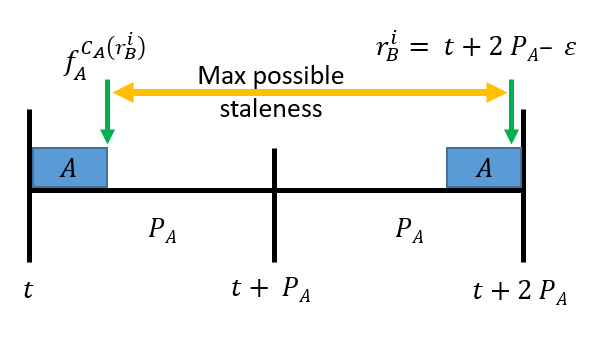
\includegraphics[width=0.3\textwidth]{figures/2TaskMaxStaleness}
	\caption{Maximum Staleness Scenario for Data from Task A.}
	\label{fig:2Tasks}
\end{figure}

Figure \ref{fig:2Tasks} labels the maximum separation between two publishes of output data from the depicted task. To maximize the staleness, we assume a job of task $B$ is released arbitrarily close to the finish of the second job of task $A$ and that the first (BCET) job of task $A$ ran to completion at the beginning of the previous period.

Note that we assume deadlines are equal to periods. However, it is easy to see here that a shorter deadline moves the latest possible execution of the second job of task A earlier, and hence decreases the max possible staleness. We will not consider this case further but it will be clear later how this could be substituted in place of our equal period and deadline example.

\begin{theorem}
	\label{thm:2TaskMaxWaiting}
	The scenario in Figure~\ref{fig:2Tasks} is the upper bound scenario for data freshness for data produced by a task.
\end{theorem}

\begin{proof}
	Note that one job must be executed within each period as per the definition of periodic tasks and our assumption of task set schedulability. Consider any placement of two jobs of a task within two consecutive periods. Assume this instance is not the one depicted in Figure~\ref{fig:2Tasks}. Then at least one of the following apply:
	\begin{case}
		The job in the first period is not completed as soon as possible. In this case, move the start of this job execution $\epsilon$ earlier. This increases the staleness by $\epsilon$.
	\end{case}
	\begin{case}
		The job in the second period is not completed as late as possible. In this case, move the start of this job execution $\epsilon$ later. This increases the staleness by $\epsilon$.
	\end{case}
	Since all other instantiations of the problem can be moved closer to the depicted instance while strictly increasing data staleness, it follows that the depicted instance is the unique worst case for output data staleness.
\end{proof}

Now that we have proven the above scenario is the worst case with regards to the freshness of data from task $A$, we can use algebra to solve for the constraint on $P_A$. From Figure~\ref{fig:2Tasks} we can see that the maximum staleness is composed of two periods of $A$ less one execution time of $A$ less $\epsilon$. We want this to be less than our freshness bound $d_{A \to B}$. We can then solve for $P_A$ to prove the following lemma.

Note that we assume the best case execution time and data delay for the first job in order to maximize staleness. The execution time of the second job is irrelevant.

\begin{lemma}
	\label{lem:2TaskResult}
	To ensure the output of task $A$ is always at most $d_{A \to B}$ old, choose $P_A \leq \frac{d_{A \to B} + E^{l,min}_A}{2}$.
\end{lemma}

\begin{proof}
	\begin{align*}
		d_{A \to B}&\geq 2P_A-E^{l,min}_A-\epsilon &\mbox{From Figure \ref{fig:2Tasks}}&\\
		P_A&\leq \frac{d_{A \to B} + E^{l,min}_A + \epsilon}{2} &\mbox{Rearrange}&\\
		P_A&\leq \frac{d_{A \to B} + E^{l,min}_A}{2} &\mbox{$\epsilon \to 0$}&
	\end{align*}
\end{proof}

We can justify bringing epsilon to zero as this is decreasing the period value and hence strictly increasing freshness. Thus if we set $P_A$ equal to the the above quantity we ensure that the output of task $A$ is always at most $d_{A \to B}$ old, and therefore can never be older when consumed by task $B$. We can also set $P_A$ less than this quantity and maintain the freshness guarantee.

Recall that our fitness metric is total utilization. It is trivial to see that choosing $P_A$ as large as possible will minimize the task set utilization. Thus the solution for the two task scenario while minimizing utilization is to set $P_A$ equal to the quantity in the lemma.

\section{Three Task Result}

We now extend the above idea to three tasks. In this scenario, let our tasks be denoted as $A$, $B$, and $C$. Task $A$ produces output consumed by task $B$, which in turn produces output consumed by task $C$. We want to limit the age of the output of $A$ that is eventually used by $C$.

For this scenario, define $d_{A \to C}$ as the maximum age of the data produced by task $A$ that is used by task $C$. Note that we are not making any assumptions about when a job of task $B$ is executed between jobs of tasks $A$ and $C$. The formalization is similar to the two task scenario:

\begin{equation*}
	\begin{aligned}
		& \text{Given:}
		& & E^{*,*}_A, E^{*,*}_B, E^{*,*}_C, P_C \text{ and } d_{A \to C} \\
		& \text{Find:}
		& & P_A \text{ and } P_B \\
		& \text{That Minimizes:}
		& & U(T) = \sum_i \frac{E_i^{u,max}}{P_i} \\
		& \text{Subject To:}
		& & 
	\end{aligned}
\end{equation*}
\begin{equation*}
	\forall i, r^i_C - f_B^{C_B(r^i_C)} + E^{u,max}_B + r_B^{C_B(r^i_C)} - f_A^{C_A(r_B^{C_B(r^i_C)})} \leq d_{A \to C}
\end{equation*}

\noindent Note that we assume worst case execution and data delay for task $B$. This will produce a more urgent local deadline that will enforce freshness also when this does not occur. More rigorously, let $\delta = E_B^{u,max} - E_B^{l,min}$. Using the max value as we do instead of the least value decreases $d_{B \to C}$ by $\delta$. As can be seen from Lemma~\ref{lem:2TaskResult} this decreases $P_B$ by $\delta / 2$. Viewing task $B$ and $C$ alone as their pair, it is easier to see that the freshness is made of two periods of $B$ for a total decrease of $\delta$. Hence, in the case of minimal execution of task $B$ the execution increases by $\delta$ but this same amount has already been compensated for in the formulation.

The execution of the three tasks is outlined in the figure \ref{fig:3Tasks}.

\begin{figure}[!ht]
	\centering
	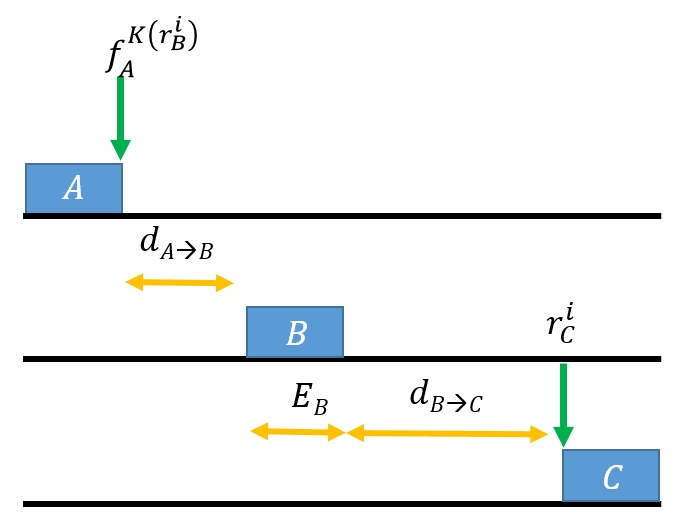
\includegraphics[width=0.3\textwidth]{figures/3TaskMaxStaleness}
	\caption{Maximum Staleness Scenario for Data from Task A.}
	\label{fig:3Tasks}
\end{figure}

Figure~\ref{fig:3Tasks} labels the several intervals in the execution of the three tasks. Note how between tasks $A$ and $B$ and between tasks $B$ and $C$ we've added local freshness constraints. By meeting these two freshness constraints, the freshness of data from task $A$ to task $C$ is ensured. These added constraints will not be present in our final solution but are added here to allow us to introduce Lemma~\ref{lem:2TaskResult} while considering task $B$. These local constraints are used as free variables in our optimization, and once determined we will use our lemma to calculate period assignments that rely only on the end-to-end constraint and task execution times.

From Figure~\ref{fig:3Tasks} we can see that the maximum age of the data from task $A$ used by task $C$, $d_{A \to C}$, is the sum of three values. Concretely,

\begin{center}
	$d_{A \to C} = d_{A \to B} + E^{u,max}_B + d_{B \to C}$
\end{center}

We now use our lemma to extend the two task result to this scenario. Using Lemma \ref{lem:2TaskResult}\ldots

\begin{center}
	$P_A \leq \frac{d_{A \to B} + E^{l,min}_A}{2} \text{ and } P_B \leq \frac{d_{B \to C} + E^{l,min}_B}{2}$
\end{center}

Our lemma uses the BCET for the first task in each pair in order to maximize the possible staleness. For our freshness guarantee, we will use the BCET to be pessimistic with the data age, whereas when calculating utilization we will use the WCET. That is, our solution will ensure freshness even in with best-case execution of the first task, while minimizing the maximum utilization the system could experience.

We simplify the objective by removing constants from the utilization expression and then transform it by substituting from Lemma~\ref{lem:2TaskResult}, using equality since lower periods increase utilization:

\begin{align*}
	U(T) &= \left(\frac{E^{u,max}_A}{P_A} + \frac{E^{u,max}_B}{P_B}\right) &\mbox{Objective}&\\
	&= \left(\frac{E^{u,max}_A}{\frac{d_{A \to B} + E^{l,min}_A}{2}} + \frac{E^{u,max}_B}{\frac{d_{B \to C} + E^{l,min}_B}{2}}\right) &\mbox{Substitution}&\\
	&= \frac{2E^{u,max}_A}{d_{A \to B}+E^{l,min}_A} + \frac{2E^{u,max}_B}{d_{B \to C}+E^{l,min}_B} &\mbox{Simplification}&
\end{align*}

We minimize this objective to arrive at the following solution.

\begin{theorem}
	\label{thm:3TaskResult}
	Given $E^{*,*}_A$, $E^{*,*}_B$, $E^{*,*}_C$, and $P_C$, to minimize utilization while enforcing the freshness bound $d_{A \to C}$, choose
	\begin{align*}
		P_A &= \frac{\sqrt{\frac{E^{u,max}_A}{E^{u,max}_B}}(E^{l,min}_B+d_{A \to C}-E^{u,max}_B+E^{l,min}_A)}{2(1+\sqrt{\frac{E^{u,max}_A}{E^{u,max}_B}})}\\
		P_B &= \frac{\sqrt{\frac{E^{u,max}_A}{E^{u,max}_B}}(E^{l,min}_A+E^{l,min}_B)+d_{A \to C}-E^{u,max}_B+2E^{l,min}_B}{2(1+\sqrt{\frac{E^{u,max}_A}{E^{u,max}_B}})}
	\end{align*}
\end{theorem}

\begin{proof}
	This optimization can be solved using elementary calculus methods. We will use Lagrangian multipliers to optimize the local constraints and then use Lemma~\ref{lem:2TaskResult} to assign periods.
	
	First we set up the Legrangian optimization problem:
	\begin{center}
		$\frac{2E^{u,max}_A}{d_{A \to B}+E^{l,min}_A} + \frac{2E^{u,max}_B}{d_{B \to C}+E^{l,min}_B} + \lambda (d_{A \to C}-d_{A \to B}-E^{u,max}_B-d_{B \to C})$
	\end{center}
	
	We now take partials with respect to our free variables, $d_{A \to B}$ and $d_{B \to C}$, and then set the partials equal to zero to solve for $\lambda$:
	
	%\begin{center}
	%	$\frac{\partial}{\partial d_{A \to B}} = -\frac{2 E^{u,max}_A}{(E^{l,min}_A+d_{A \to B})^2}-\lambda
	%	\text{ and }
	%	\frac{\partial}{\partial d_{B \to C}} = -\frac{2 E^{u,max}_B}{(E^{l,min}_B+d_{B \to C})^2}-\lambda$
	%\end{center}
	
	%We set these equal to zero and solve for our $\lambda$'s \ldots
	\begin{align*}
	-\frac{2 E^{u,max}_A}{(E^{l,min}_A+d_{A \to B})^2}-\lambda &= 0 \to \lambda = -\frac{2 E^{u,max}_A}{(E^{l,min}_A+d_{A \to B})^2}\\
	-\frac{2 E^{u,max}_B}{(E^{l,min}_B+d_{B \to C})^2}-\lambda &= 0 \to \lambda = -\frac{2 E^{u,max}_B}{(E^{l,min}_B+d_{B \to C})^2}
	\end{align*}
	
	With two values of $\lambda$ we can form an equality which we can use with our constraint equation in a system of equations to solve for $d_{A \to B}$ and $d_{B \to C}$. We'll solve for $d_{A \to B}$ first:
	
	%\begin{align*}
	%	-\frac{2 E^{u,max}_A}{(E^{l,min}_A+d_{A \to B})^2} &= -\frac{2 E^{u,max}_B}{(E^{l,min}_B+d_{B \to C})^2}\\
	%	d_{A \to B}+E^{u,max}_B+d_{B \to C} &= d_{A \to C}
	%\end{align*}
	
	%We'll solve for $d_{A \to B}$ first.
	
	\begin{align*}
		&-\frac{2 E^{u,max}_A}{(E^{l,min}_A+d_{A \to B})^2} = -\frac{2 E^{u,max}_B}{(E^{l,min}_B+d_{B \to C})^2} &\mbox{}&\\
		& \mbox{Rearrange for $d_{A \to B}$:} & &\\
		%&(E^{l,min}_A+d_{A \to B})^2 = \frac{E^{u,max}_A}{E^{u,max}_B}(E^{l,min}_B+d_{B \to C})^2 &\mbox{}&\\ %Rearrange and Simplify
		d_{A \to B} &= \pm\sqrt{\frac{E^{u,max}_A}{E^{u,max}_B}} \left(E^{l,min}_B+d_{B \to C}\right)-E^{l,min}_A &\mbox{}&\\ %Isolate variable
		& \mbox{Substitute Rearranged Constraint:} & &\\
		&=\pm\sqrt{\frac{E^{u,max}_A}{E^{u,max}_B}} \left(E^{l,min}_B+d_{A \to C}-E^{u,max}_B-d_{A \to B}\right)-E^{l,min}_A &\mbox{}&\\ %Substitute From Constraint
		& \mbox{Rearrange to remove $d_{A \to B}$ from right side:} & &\\
		&=\frac{\pm\sqrt{\frac{E^{u,max}_A}{E^{u,max}_B}} (E^{l,min}_B+d_{A \to C}-E^{u,max}_B)-E^{l,min}_A}{1+\pm\sqrt{\frac{E^{u,max}_A}{E^{u,max}_B}}} &\mbox{}& %Simplify
	\end{align*}
	
	We obtain two possible solutions, one where both $\pm$ are set to $+$ and another where they are set to $-$ (they remain consistent as they were produced by the same root operation).
	
	%\begin{align*}
	%	d_{A \to B}&= \frac{\sqrt{\frac{E^{u,max}_A}{E^{u,max}_B}}(E^{l,min}_B+d_{A \to C}-E^{u,max}_B)-E^{l,min}_A}{1+\sqrt{\frac{E^{u,max}_A}{E^{u,max}_B}}}
	%	\text{ or}\\
	%	d_{A \to B}&= \frac{-\sqrt{\frac{E^{u,max}_A}{E^{u,max}_B}}(E^{l,min}_B+d_{A \to C}-E^{u,max}_B)-E^{l,min}_A}{1-\sqrt{\frac{E^{u,max}_A}{E^{u,max}_B}}}&
	%\end{align*}
	
	Note we can drive utilization arbitrarily higher by shortening the local constraints, hence there is no maximum in our search space. There are also no saddle points: it is clear that from any initial value, increasing either parameter will strictly lower utilization. It follows that both of these points are minima. Now note that the potential solution with $-$'s obtains optimality by using negative values which are out of our domain. Upon inspection its easy to see how $d_{A \to B}$ can become negative when $E_A^{u,max} > E_B^{u,max}$, and is undefined when these two are equal. Since our local constraints must be positive, this is not a feasible solution and we discard it.
	
	And now we solve for $d_{B \to C}$ using the feasible ($+$'s) solution and the constraint equation:
	
	\begin{center}
		$d_{B \to C} = d_{A \to C} - E^{u,max}_B- \frac{\sqrt{\frac{E^{u,max}_A}{E^{u,max}_B}}(E^{l,min}_B+d_{A \to C}-E^{u,max}_B)-E^{l,min}_A}{1+\sqrt{\frac{E^{u,max}_A}{E^{u,max}_B}}}$
	\end{center}
	
	We can now use Lemma~\ref{lem:2TaskResult} to convert these into periods:
	
	\begin{align*}
		P_A &= \frac{\sqrt{\frac{E^{u,max}_A}{E^{u,max}_B}}(E^{l,min}_B+d_{A \to C}-E^{u,max}_B)-E^{l,min}_A}{2(1+\sqrt{\frac{E^{u,max}_A}{E^{u,max}_B}})}+ \frac{E^{l,min}_A}{2}\\
		P_B &= -\frac{\sqrt{\frac{E^{u,max}_A}{E^{u,max}_B}}(E^{l,min}_B+d_{A \to C}-E^{u,max}_B)-E^{l,min}_A}{2(1+\sqrt{\frac{E^{u,max}_A}{E^{u,max}_B}})} \\&+\frac{d_{A \to C}-E^{u,max}_B+E^{l,min}_B}{2}
	\end{align*}
	
	These simplify to the values provided in the theorem statement. This concludes our proof.
\end{proof}

This is a convex optimization problem where we can always find arbitrarily small periods that meets our freshness bound, i.e. we always have an interior point that satisfies our constraint and thus the problem is strictly feasible. It follows that this problem has strong duality and our solution are our desired parameters.

As intended, our solution is expressed solely in terms of the task parameters and the end-to-end freshness requirement. The formulation may assign non-integer periods which we consider acceptable. The designer could floor such values to the nearest platform-compatible value while preserving the freshness guarantee. If the designer is concerned about a large number of tasks in the system, several tasks with similar periods could be combined into one task with the lowest period of the component tasks. However, both of these modifications will increase utilization.

This solution may not be schedulable. In the case it is not, there may be a schedulable parameter set that guarantees the desired freshness, depending on the system's scheduling policies. Finding the optimal parameters in such a case may be non-trivial.

It may be possible to extend this optimization to more tasks. Using the same notation one could craft calculus minimization problems for a given number of tasks. The primary challenge would be solving increasingly difficult optimization problems. It may be possible to generalize this method to $n$ tasks in this manner. However, moving forward we will express the formulation as a general optimization problem to be solved with a software solver.
\section{Discussion}

We note several issues with this approach. For one, it generalizes for any scheduling algorithm. Given information about the scheduling algorithm, prioritization, and preemptability, one could likely produce parameters that result in lower utilization. For many schedulers this would mean larger periods for our input tasks than presented in our solution.

The most important limitation to note, as mentioned several times already, is that this method does not guarantee the schedulability of the task set. This is due to its scheduler agnosticism. However, this is easily remedied by scheduler-specific schedulability tests. A weak, universal, necessary assessment would be to check if the utilization is less than 1, since we are considering a uniprocessor system. If the particular value produced by this method is unschedulable, there may or may not exist other parameters that schedule the task set while ensuring freshness for a given scheduler. This becomes particularly difficult if extended to multicore systems.

It may be possible to extend this model further to even more tasks. Using the same notation as used for the three task model, one could craft complex minimization problems for a given number of tasks. The primary challenge would then be solving increasingly difficult optimization problems. It may be possible to generalize this method to $n$ tasks but this has not yet been pursued.
\section{Related Work}
Others have investigated proper period selection for tasks. However, most opt to consider a specific scheduler or other assumptions about the task set, or don't consider data freshness as the end goal. [To be expanded]
\section{Conclusion}

In this paper we considered the freshness of data consumed by tasks within a periodic task system. We aimed to select the periods of input tasks in order to ensure the freshness of data consumed later chain tasks. Without assumptions regarding the scheduler, we proved upper bounds on the periods of tasks in order to ensure the freshness of data through chains of tasks of length two and three for uniprocessor systems. We then extended the theory to an optimization problem suitable for any chain length and configuration.

%\end{multicols}

\newpage
{\footnotesize \bibliographystyle{acm}
	\bibliography{references}
}

\appendix

\end{document}
